In the seminal paper by Einstein \cite{einsteinUberErzeugungUnd1905}, that laid foundations to Quantum Mechanics, Einstein postulated that light is made of discrete quanta of energy $E = h\nu$ to explain the observations by Hertz and J.J. Thompson; explaining the photoelectric effect. The effect can be described by the Equation \ref{eq:photoelectric} where $E_e$ the emitted kinetic energy, $h$ is the Planck's constant, $\nu$ the frequency of the incoming photon and  $\phi$ the material-specific work function (also known as binding energy). 

\begin{equation}\label{eq:photoelectric}
    E_e = h\nu - \phi
\end{equation}

The equation describes how incident photons on a surface eject photoelectrons, provided the photon energy $h\nu$ exceeds $\phi$.
It is then apparent that the binding energy of electrons can be found by irradiating light onto the material and measuring the $E_e$ of photoelectrons. \Gls{PES}, is exactly such a technique that leverages this principle to probe the electronic structure of materials.

\cref{eq:photoelectric} also highlights that the emitted kinetic energy $E_e$ is dependent on the photon energy but independent of the photon flux (photons per second). However, the flux of photons does affect the number of photoelectrons emitted. This effect and the probabilistic nature of the photoemission process can only be described with the quantum theory of light-matter interaction\footnote{Many of the results can be explained by semi-classical theory as well, which treats the light as a classical wave and the electrons as quantum particles.}.

The whole process of excitation, transport, and emission can be treated as a single coherent process using the formalism of quantum mechanics. This approach incorporates the electronic structure, electron-electron interactions, and the surface barrier in a unified way, and describes the photoemission intensity  $I(E, k_x, k_y)$ being proportional to probability.

The process can be described by the Fermi's Golden Rule, which gives the transition rate between two states. In the context of photoemission, the initial state is the electron in the material, and the final state is the electron in the vacuum. The intensity of photoemission can be then described by the transition rate between the two states, and the energy conservation:

\begin{equation}
    I(E, k_x, k_y) \propto |\langle \psi_f | \mathbf{A} \cdot \mathbf{p} | \psi_i \rangle|^2 \delta(E - E_f)
\end{equation}
where $\psi_i$ and $\psi_f$ represent the initial and final electron wavefunctions, $\mathbf{A} \cdot \mathbf{p}$ is the matrix element that couples the photon to the electron, and the $\delta$ function ensures energy conservation between the initial and final states.

In the linear regime, an increase of photon flux results in increased photoemitted electrons (or vise versa), but not in $E_e$. However, at high photon fluxes, non-linear photoemission processes start playing a more significant role. In such a case, an electron is emitted after absorbing more than one photon, leading to a deviation from the single-photon flux relation. 

A variety of photoemission spectroscopy methods can be devised depending on which parameters are varied and what is measured. Naturally, the most basic setup would measure the energy of the emitted electron as described in equation \ref{eq:photoelectric}, while variations of the technique allow for additional parameters, such as resolving the electron momentum and spin, or dynamics.

\Gls{ARPES} measures both the kinetic energy $E_e$ and the parallel momentum components (\gls{kx}, \gls{ky}) of the emitted electrons. By varying the photon energy, \gls{ARPES} can also provide information on the surface perpendicular momentum component \gls{kz}. \Gls{XPS} focuses on the core-level electrons, providing information on the chemical composition and oxidation states of atoms in a material. By analyzing the binding energies of core electrons, \gls{XPS} can offer insights into the local electronic environment of atoms. \Gls{trPES} takes this process a step further by probing the dynamics of electronic states, allowing to understand transient, non-equibilrium phenomena. A pump-probe scheme is usually employed, where a pump laser drives the system out of equilibrium, and the core- or valence-electron states are probed by a probe laser. By applying an offset between the two pulses, the dynamics of the electronic states can be studied as a function of time.

As many of the interesting dynamics happen on the ultrafast timescale, on the order of \unit{fs} to \unit{ps}, such as charge carrier dynamics, phonon dynamics, and optically induced phase transitions, it is imperative that the light source used for \gls{trPES} has a finer temporal resolution than the timescale of the phenomena being studied. We will discuss the key light sources commonly used for \gls{trPES}, namely \gls{HHG} lasers, and \glspl{FEL}.

\Glspl{FEL} are particularly well suited for \gls{trPES} due to their high peak brightness, \unit{fs} pulse durations and energy tunability. But these high fluxes come with a caveat especially in \gls{trPES}; namely the space-charge effect. This occurs when flux of photoemitted electrons is too high, inducing a coulomb repulsion between the electrons, and leading to a distortion in their trajectories and energies. We look at the compromise between the intensity of the light source and the space-charge effect, and how the \gls{HEXTOF} instrument, equipped with the \num{8}-sector \gls{DLD}, is designed to address this challenge.

Finally, we discuss the data acquisition scheme, and the experimental datasets of \gls{GrIr}, \gls{NiW}, \gls{GdW}, and \gls{WSe2} that have been studied.

\section{Light Sources}\label{section:light-sources}
We have seen that the radiation source plays a critical role in both \gls{PES} and \gls{trPES}. Monochromatic\footnote{Truly monochromatic radiation is physically impossible, and generally a range is considered.} \gls{XUV} energy and high repetition rate sources are necessary to probe only the relevant systems, and acquire large amount of data quickly. \Gls{trPES} further requires the source to be temporally coherent, with pulse durations on the order of femtoseconds.

\subsection*{Laser}
The most ubiquitous of light sources--the laser--revolutionized experimental science as it enabled a vast range of phenomena to be precisely tested and observed, due to its high spatial and temporal coherence properties. A laser produces its light through a process known as stimulated emission, a process in which electrons, excited to higher energy states by an external energy source, emit photons as they return to lower energy states. These emitted photons, in turn, stimulate other electrons to release additional photons, leading to a cascade of coherent light. A process known as \gls{HHG} is used to generate ultrafast light of higher energies so that valence and core electrons states can be probed.

% \subsection{Synchrotron}
% Particle accelerators, initially used for high energy physics experiments, which produce radiation as a byproduct of particles accelerating, found their use in spectroscopy. Soon, dedicated facilities providing extremely bright and tunable source of electromagnetic radiation emerged. One class of such facilities are known as Synchrotrons, which are named due to their cyclic design. Typically, bunches of electrons are accelerated by bending magnets, known as an \glspl{undulator}, placed around a storage ring. These electrons are accelerated till they reach appropriate energies and provide a continuous source of radiation. Tangent to the ring, at certain points in the facility are beamlines which direct the radiation to the experimental end-stations, used to perform experiments in fields of life science, material science, and medicine to name a few.

% There are several synchrotron facilities around the world, and in Germany such as BESSY II in Berlin, PETRA III at DESY campus in Hamburg.

\subsection*{Free-Electron Laser}
Particle accelerators, initially used for high energy physics experiments, which produce radiation as a byproduct of particles accelerating, found their use in spectroscopy. Soon, dedicated facilities providing extremely bright and tunable source of electromagnetic radiation emerged such as Synchrotrons and \glspl{FEL}.
While Synchrotrons are excellent sources of light for a multitude of experiments, they have limitations in terms of the temporal coherence of the light produced. \Glspl{FEL} are linear particle accelerators that produce a pulsed light source with a high temporal coherence, and energies to probe allowing core and deep valence electrons. There are two modes under which \glspl{FEL} operate: \gls{SASE} and seeded.


In \gls{SASE} mode, the amplification process is initiated by the electron shot-noise (\gls{spontaneous_emission}) when the electron beam in the accelerator passes through an undulator. Undulators are periodically arranged magnets that cause the electrons to oscillate and emit radiation. The interaction between the emitted radiation and the charge distribution leads to a phenomenon known as \gls{microbunch}. These microbunches emit radiation coherently, leading to the intense, coherent radiation, characteristic of a \gls{FEL}. 

Due to the inherent stochastic nature of the process, the radiation produces intensity fluctuations and hence a lower degree of temporal coherence. Such fluctuations can be seen using a \gls{GMD} (see glossary \gls{gmd} for details) as shown in Figure \ref{fig:gmd-intensity}. The light produced by an \gls{FEL} is of high peak brightness and can be compressed to \unit{fs} pulse durations, making it an ideal source for studying ultrafast phenomena.

To improve the temporal coherence, some \glspl{FEL} such as FERMI \cite{svandrlikDevelopmentPerspectivesFERMI2017} operate in the seeded mode, where a coherent seed laser is used to initiate the amplification process. This leads to a higher degree of temporal coherence in the light produced.

\begin{figure}
    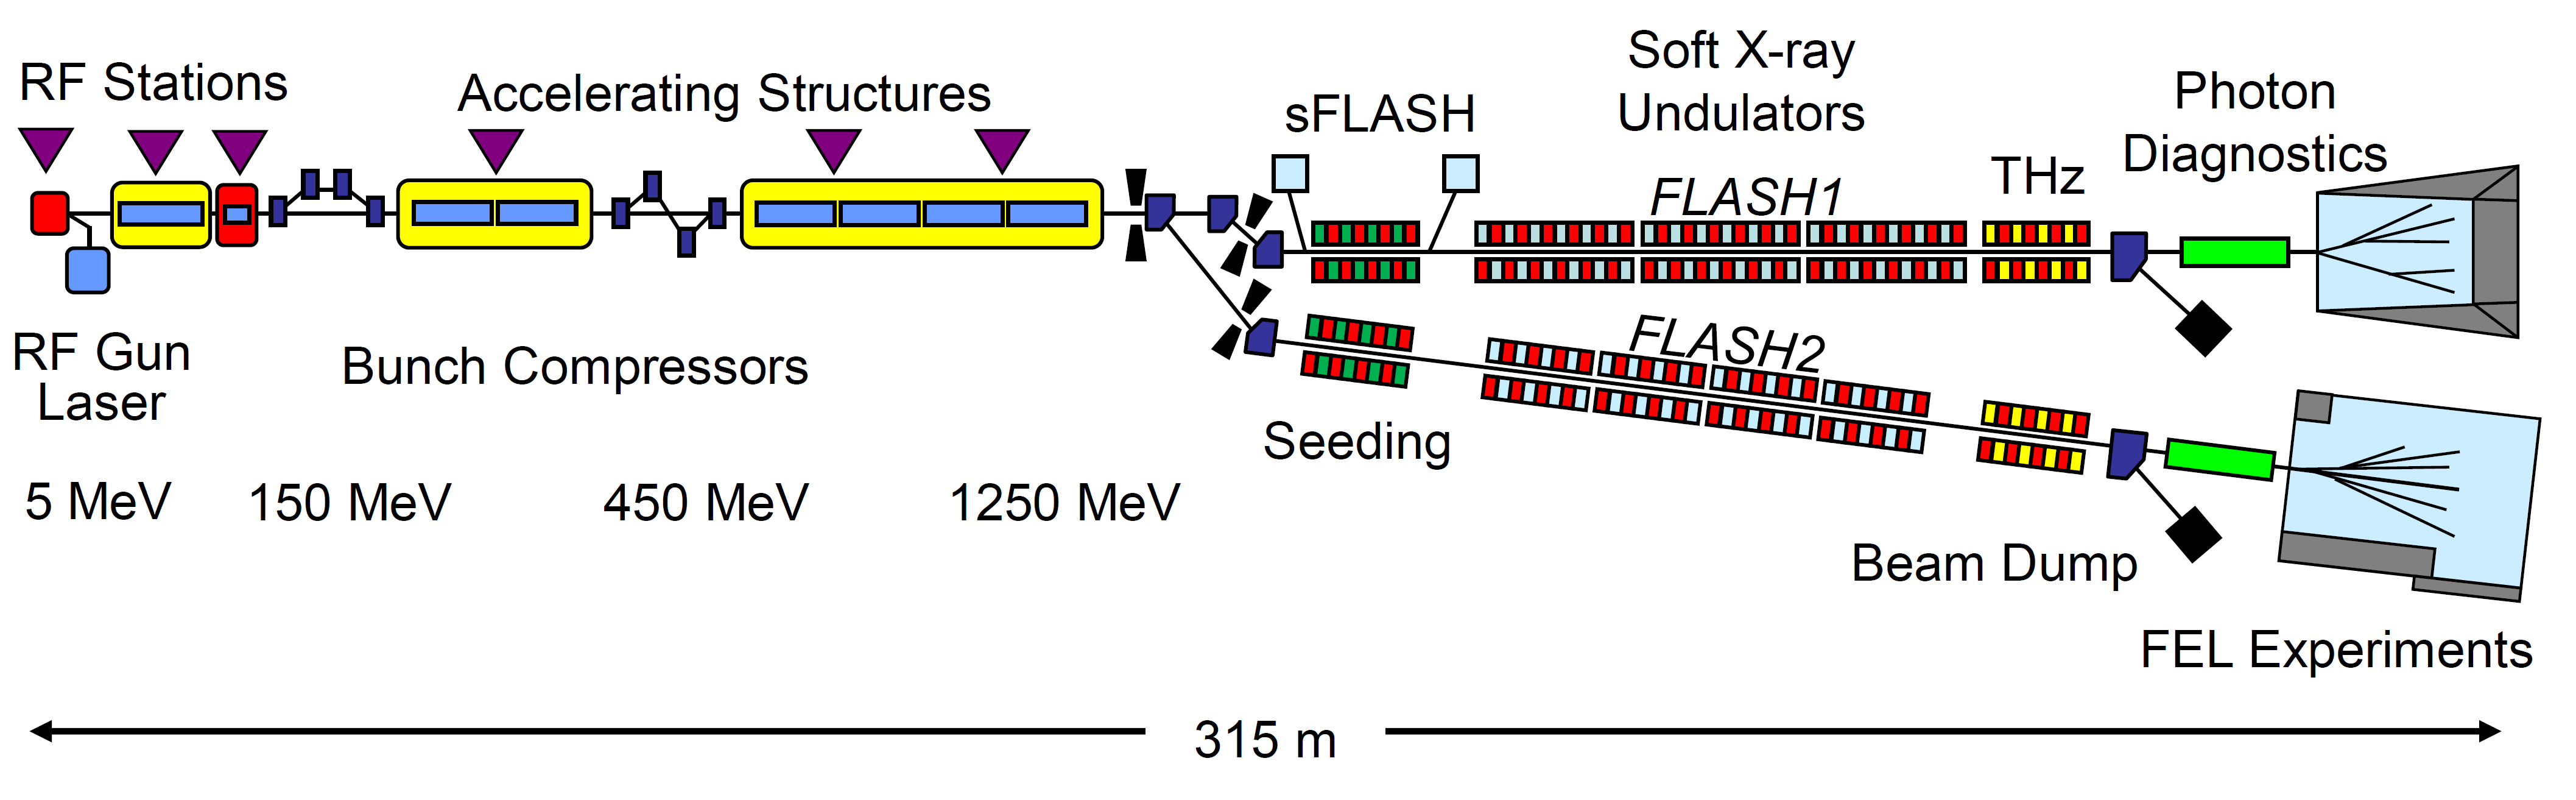
\includegraphics[width=1\linewidth]{images/flash_fel.png}
    \caption{Schematic view of \gls{FLASH} taken from \cite{faatzSimultaneousOperationTwo2016}.}
    \label{fig:flash-schematic}
\end{figure}

\gls{DESY} is a national research center in Germany that operates the \gls{FEL} \gls{FLASH} facility \cite{ackermannOperationFreeelectronLaser2007,tiedtkeSoftXrayFreeelectron2009} that produces ultrashort \gls{XUV} and soft X-ray radiation in the wavelength range of \qtyrange{4}{50}{\nm} in the fundamental, and as low as \qty{1.7}{\nm} in the third harmonic, corresponding to a total photon energy range of \qtyrange{25}{830}{\eV}. With an average pulse energy of \qtyrange{1}{500}{\micro\joule}, and pulse durations \qty{<10}{\fs}, peak powers of \qtyrange{1}{5}{\giga\watt} can be reached. This makes it an ideal source for studying ultrafast processes in materials and molecules. An example scheme of the acceleration modules, \glspl{beamline} and experimental end-stations can be seen in Figure \ref{fig:flash-schematic}, where our experiments are performed at the PG2 beamline at FLASH1 (see FLASH1 and 2 in \cref{fig:flash-schematic}).

\section{Challenges in Photoemission Spectroscopy}
With the inherent stochastic nature of the photoemission process, the only way to resolve the electronic structure with high precision is to average many events to approach the expected value, as individual measurements fluctuate around the expected value. For a constant intensity light source, the standard deviation of the measurements decreases as the square root of the number of events. This does not hold for a fluctuating source, which is prone to higher fluctuations. 

To ensure the statistical significance of time-resolved studies, the repetition rate and flux of the radiation source need to be high enough to capture non-linear effects\footnote{Nonlinear effects, such as multiphoton processes, are rare and require high flux to observe.}, to probe excited electronic states with low population densities etc. While \glspl{FEL} like \gls{FLASH} are well suited for such experiments, having a high flux can be detrimental for \gls{PES} due to the phenomenon known as the space-charge effect.

The space-charge effect occurs when intense light pulses generates a large electron density. This leads to the Coulomb repulsion between electrons, causing a distortion in the electric field, leading to a spread in the energy of the electrons\footnote{Effectively reducing the energy and momentum resolution.}. This effect is more critical in time-resolved experiments, as the pumping laser also induces an excitation. To mitigate this, the intensity of the light source must be attenuated, and the most efficient detection schemes must be used in combination with high repetition rate sources.

As can be seen on the top left of \cref{fig:hex-tof}, \gls{FLASH} provides a very high repetition rate of \qty{1}{\mega\hertz} or \qty{1}{\micro\second} gap between \glspl{pulse}. However, there are about 500 pulses in each \gls{train}, and the \gls{FEL} operates at \qty{10}{\Hz} or \qty{100}{\milli\second} between trains, having an effective rate of \num{5000} probe pulses per second. This suggests that there are no measurements over half the time. 

Efficient detection schemes are then necessary to capture all emitted electrons as not only is the repetition rate relatively low, the flux is also attenuated to be below the space-charge limit. Electron counting detectors typically have a dead-time, meaning that after a measurement, the detector is unable to detect another electron for a certain period of time. This dead-time can be longer than a pulse duration, so detection is less than an electron every pulse. More sophisticated detection schemes are then necessary to capture more emitted electrons, and reduce the acquisition time; a topic in the next section.

\section{Detection Systems: Time-of-Flight Momentum Microscope with a Multi-Sector Delay Line Detector}
The \gls{HEXTOF} instrument shown in \cref{fig:hex-tof} is designed to perform core- and valence-electron time- and momentum-resolved studies at \gls{FLASH}, addressing challenges such as low-repetition-rate sources, and the space-charge effect. The instrument combines a \gls{DLD} with a \gls{TOF} tube to detect individual electrons and measure their momentum and kinetic energy simultaneously.

One of the standout features of \gls{HEXTOF} is its multidimensional recording scheme. This approach allows for simultaneous measurement of multiple parameters that can be related to the complete momentum space \gls{kx}, \gls{ky}, \gls{kz}, energy \gls{E}, and delay time \gls{tpp}. The \gls{kx} and \gls{ky} are recorded based on the direction of the emitted electrons, while the \gls{kz} is determined by tuning the photon source. The \gls{E} is determined by the time-of-flight of the electrons, and the \gls{tpp} is the delay between the pump and probe pulses. More recently, the spin branch has been explored and spin polarization \gls{Sz} added to the list of parameters that can be measured. 

\begin{figure}
    \centering
    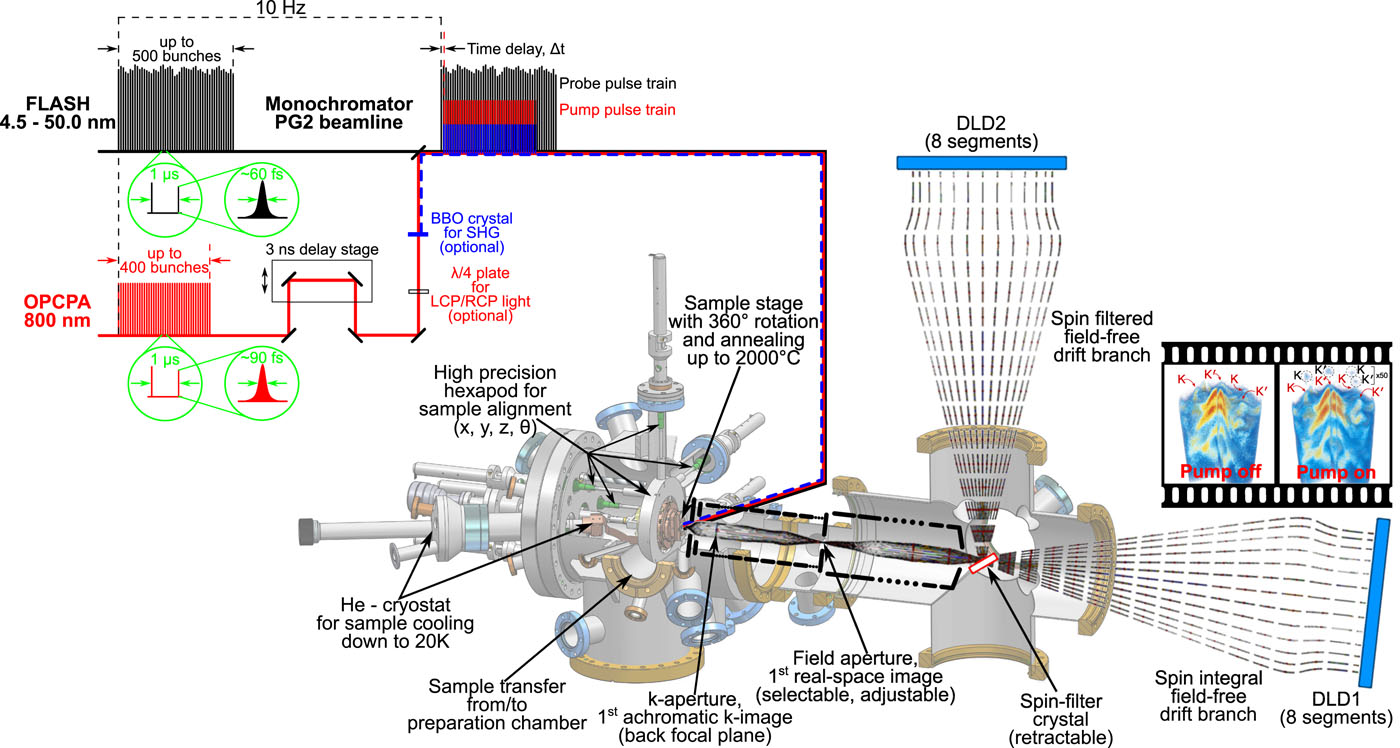
\includegraphics[width=1\linewidth]{images/2024-08-27-10-50-01.png}
    \caption{The \gls{FLASH} pulse structure and the \gls{HEXTOF} experimental setup. Taken from \cite{kutnyakhovTimeMomentumresolvedPhotoemission2020}.}
    \label{fig:hex-tof}
\end{figure}


\subsection{Delay Line Detectors}\label{section:dld}
Individual electrons released by the photoemission process are difficult to directly detect due to their low energies. \Glspl{MCP} are amplifiers of sort (electron multipliers), that generate a cascade of secondary electrons when an electron strikes the detector surface. This amplification allows for the detection of individual electrons. \Glspl{MCP} generally do not resolve for position of electrons and schemes such as \gls{MCP} combined with a delay-line readout are used to determine the position. 

The readout consists of a series of meandering\footnote{This zigzag pattern increases effective length, allowing for finer temporal resolution and hence position.} wires running in orthogonal directions beneath the \gls{MCP}. The cloud of electrons can then be detected by the delay-line readout and the signal travels along the wires connected to a series of precise timing circuits. Using \glspl{TDC}, The time difference for the signal to travel from the point of impact to the readout is used to determine the position of the electron.


The \gls{TOF} tube built into the \gls{HEXTOF} instrument is used to measure the time electrons take to travel from the sample to the detector. The \gls{TOF} can be measured by recording the initiation of the event (when the photon pulse comes) till when they hit the \gls{MCP}. Since electrons with different energies travel at different velocities, the \gls{TOF} can be used to determine the kinetic energy of the electrons. 

The detector is divided into \num{4} quadrants, each able to detect electrons independently. This division allows the system to detect several electrons from the same or different pulses without significant dead-time. While the quandarant structure ensures higher detection, if and electron has momenta that falls in a quadrant which is already detecting an electron, the dead-time can lose the second electron. That is why the \gls{DLD} has a multi-layer structure as seen in \cref{fig:sectors}, where the two layers are stacked at \qty{45}{\degree} to each other. This allows for detection of events that might fall on the same quadrant space.

\begin{figure}[h]
    \centering
    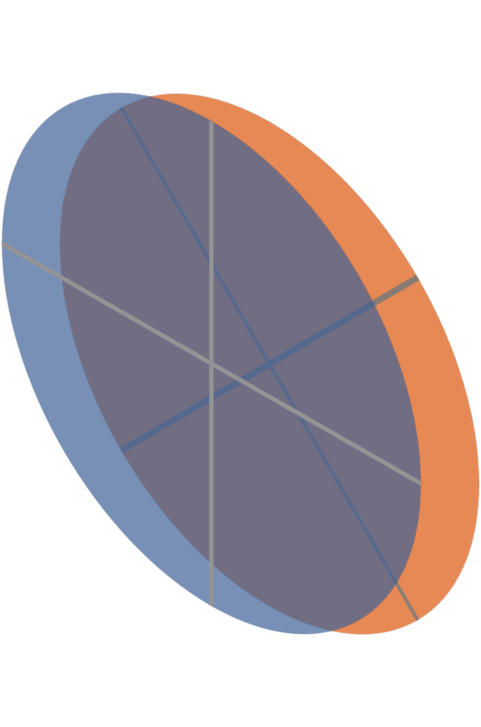
\includegraphics[width=0.3\linewidth]{images/sectors_figure.pdf}
    \caption{Schematic of the 2-layered DLD. The detector is divided into 2 layers, each with 4 sectors.}
    \label{fig:sectors}
\end{figure}

Owing to the 2-layered \gls{DLD} in our experimental setup, measuring two electrons impinging on locations nearby to one another can be detected. However, the multi-layer detection scheme comes with a caveat: the layers must be calibrated appropriately otherwise the electron counting routines can report two or more events for the same electron (due to the angle between the layers); with different momenta due to the miscalibration. With a correlation analysis on the photoelectrons generated in pulses, this effect has been observed by [Haber Thesis here]. This multiple counting also occurs within the individual layers, at the intersection of individual sectors.

This effect not only wrongly counts electrons but also distorts (blurs) the momentum distribution. \citeauthor{heberStudiesUltrafastDynamics2024} further demonstrates that by first finding the double-counted events (or more) and averaging them, the resolution of the momentum distribution can be improved as can be seen in \cref{fig:chessy-distribution} right.

%images/chessy_deblurring_merged_events.png
\begin{figure}[h]
    \centering
    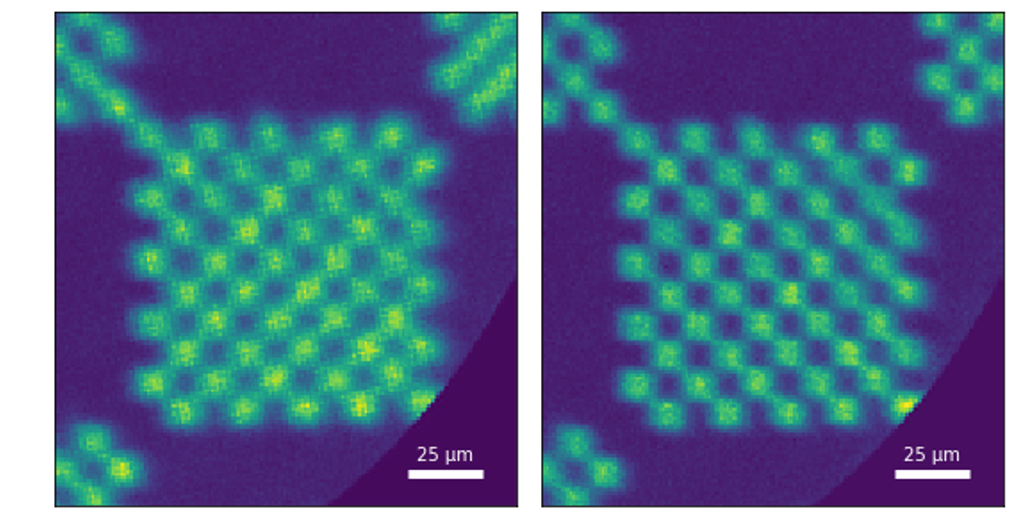
\includegraphics[width=0.7\linewidth]{images/chessy_deblurring_merged_events.png}
    \caption{Chessy sample before and after merging double-counted events. It can be seen that the momentum distribution is improved after averaging over the double-counted events. Taken from \cite{heberStudiesUltrafastDynamics2024}.}
    \label{fig:chessy-distribution}
\end{figure}


It has also been observed that the \gls{DLD} codes can not always accurately reconstruct the events, due to signal overlap, such as in the study by \citeauthor{knipferDeepLearningbasedSpatiotemporal2024}. They have proposed a deep learning based method to reconstruct the events accurately \cite{knipferDeepLearningbasedSpatiotemporal2024}.

\section{Experimental Datasets}\label{section:datasets}
We look at four materials that have been studied using \gls{HEXTOF} at \gls{FLASH}: \gls{GrIr}, \gls{NiW}, \gls{GdW}, and \gls{WSe2}. Long acquisition times are necessary to get interpretable results. This is due to three main reasons. As mentioned above, the intrinsic stochastic nature of the photoemission process requires us to collect a large number of events to approach the true value (expected value). Additionally, the low repetition rate of the \gls{FEL} means that we need to collect data over a long period of time to get enough events. Lastly, the multidimensional acquisition scheme to simultaneously resolve \gls{kx}, \gls{ky}, \gls{kz}, \gls{E}, \gls{tpp}, and \gls{Sz} suffers from the curse of dimensionality. With an increase in dimension, the space becomes sparser, and exponentially more data is needed to fill the space.

\begin{figure}[h]
    \centering
    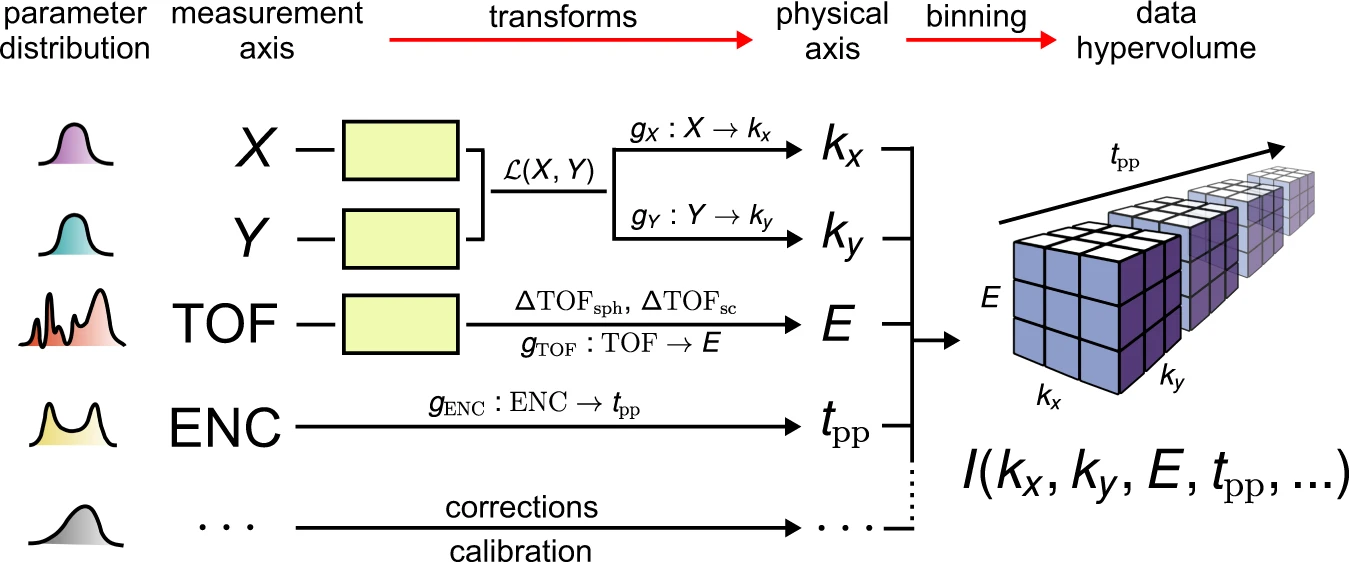
\includegraphics[width=1\linewidth]{images/41597_2020_769_Fig2_HTML.png}
    \caption{A typical workflow for a \gls{trPES} experiment. Taken from \cite{xianOpensourceEndtoendWorkflow2020}.}
    \label{fig:mpes_workflow}
\end{figure}

For a \gls{trPES}, a common workflow is shown in \cref{fig:mpes_workflow}, where the measurement axes is first mapped to the  physical axes and the single-event data is binned into a multidimensional volume. For an in depth description of how data is extracted and transformed, please refer to Appendix~\ref{sec:elt}.

\begin{figure}
    \centering
    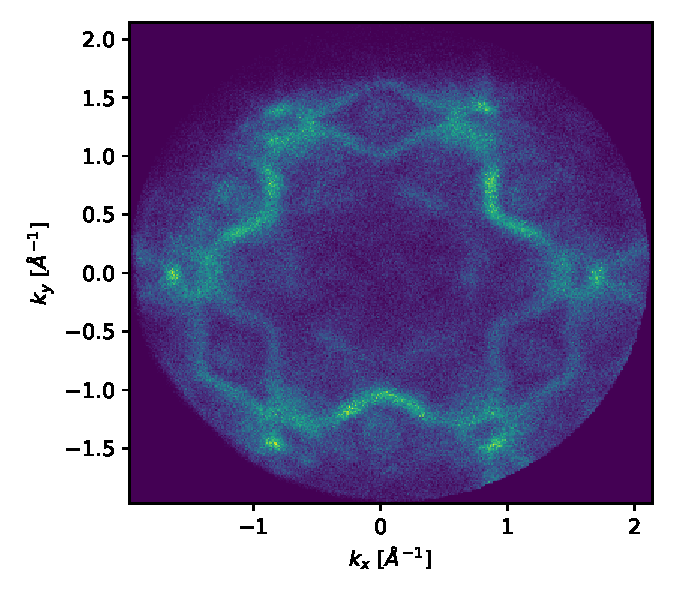
\includegraphics[width=0.5\linewidth]{images/calibrated_momentum.pdf}
    \caption{2D slice (window-averaged over the energy dimension) of the \gls{GrIr} dataset in the \gls{ky}--\gls{kx} plane. The data has been calibrated to map the pixel values to the physical momentum axes.}
    \label{fig:grir-2d-slice-calibrated}
\end{figure}

\begin{figure}[h]
    \centering
    \includegraphics[width=1\linewidth]{images/3d_gr_ir_masked.png}
    \caption{A 3D image constructed from the \gls{GrIr} dataset. The image is constructed by binning over the three physical axes $k_x$, $k_y$, $E$ from different datasets. 2D images can be formed by slicing (or window averaging) along any of the axes.}
    \label{fig:3d-gr-ir}
\end{figure}

If we just want to look at the static results, a 3D image such as \cref{fig:3d-gr-ir} can be formed by binning across the three physical axes--\gls{kx}, \gls{ky} and \gls{E}--from different datasets such as the \gls{GrIr} dataset, which contains \num{1.86e8} electron counts in the entire dataset. The average count decreases when binning across additional dimensions, such as the pump-probe time \gls{tpp} or spin polarization \gls{Sz}. After focusing on a \gls{ROI} (\gls{EF} and near), and 3D binning with a resolution of \num{512} in each direction, the total counts become \num{1.15e8}, with an average count of $\approx$1.05 per voxel. 

Slicing along the \gls{E} direction, we can form 2D images such as the one shown in \cref{fig:grir-2d-slice-calibrated}.

With the \gls{DLD} providing a stream of single-event data, we are uniquely positioned to access true noisy realizations by taking subsets of varying total electron counts from the full dataset. These subsets can then be binned to form independent 3D images, used later for evaluating and training denoising algorithms.

\begin{figure}
    \centering
    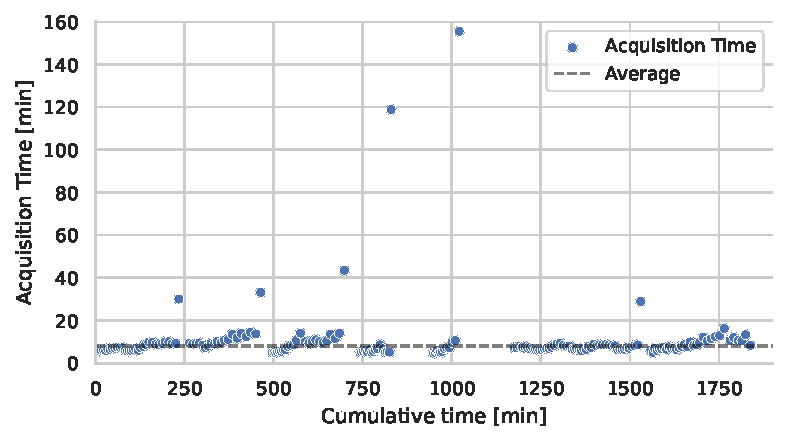
\includegraphics[width=0.8\linewidth]{images/acq_time_1M.pdf}
    \caption{Total acquisition time in minutes for generating \num{e6} data points. Some outliers are present due to the photon source being off, leading to longer acquisition times. The average acquisition time without outliers is approximately 8 minutes (see dashed line).}
    \label{fig:acq-time-1M}
\end{figure}


As seen in \cref{fig:acq-time-1M}, \num{e6} counts roughly correspond to \qty{8}{\min} of data acquisition, illustrating the total acquisition time to generate \num{e6} electron events. From the complete dataset, \num{186} subsets—sampled at one-million-count intervals—can be extracted. In theory, the data generation is an independent stochastic process, allowing for a large variety of randomly sampled subsets. However, in our case, the \gls{FEL} light source introduces a degree of dependence as it is not stable over extended periods, beyond its intrinsic fluctuations.


\begin{table}[h]
    \centering
    \resizebox{0.6\textwidth}{!}
        {%
        \begin{tabular}{lrr}
            \toprule
            & Counts & Average Counts Per Voxel \\
            &  &  \\
            \midrule
            Noisy & \num{1e6} & 0.006 \\
            Noisy & \num{2e6} & 0.011 \\
            Noisy & \num{4e6} & 0.023 \\
            Noisy & \num{8e6} & 0.046 \\
            Noisy & \num{1.6e7} & 0.091 \\
            Noisy & \num{3.2e7} & 0.183 \\
            Noisy & \num{4.8e7} & 0.274 \\
            Noisy & \num{9.6e7} & 0.546 \\
            Target & \num{1.86e8} & 1.055 \\
            \bottomrule
        \end{tabular}
        }
    \caption{Noisy realizations generated from varying total counts. The acquisition time is proportional to the total counts, with the \num{1.86e8} count dataset serving as the target.}
    \label{noisy-dataset-table}
\end{table}

Noisy realizations can then be formed based on a number of total counts. The total counts and average counts per voxel for each noisy realization are shown in \cref{noisy-dataset-table}. These realizations can help evaluate the performance of denoising algorithms as a function of acquisition time. Lower count realizations ($<$e7), corresponding to shorter acquisition times, are of most interest to denoise. Successful denoising of such data could significantly improve experimental efficiency, allowing the investigators to steer the experiment in the right direction, crucial in time-limited \glspl{beamtime}. Hence, the realizations are sampled at count values: \numlist{1e6;2e6;4e6;8e6;1.6e7;3.2e7;4.8e7;9.6e7}.


% \subsection{Calibration}
% We present an example calibration workflow to calibrate--mapping of pixel values to the momentum axes of \gls{GrIr} dataset. Graphene is a 2D material with carbon atoms arranged in a hexagonal honeycomb structure. The Brillouin zone exhibits high-symmetry points in the reciprocal lattice (momentum space) such as the $K$-point and $K'$-point, located at the corners of the hexagonal zone, and $\Gamma$-point, located at the center \cite{castronetoElectronicPropertiesGraphene2009}. The calibration process is to map the detector pixel axes to the physical momentum axes.

% In graphene's reciprocal lattice, the momentum space coordinates of the $K$-point can be derived from the lattice vectors. The reciprocal lattice vector components in the hexagonal Brillouin zone are given by:
% \begin{equation*}
%     k_x = \frac{2\pi}{3a}
% \end{equation*}
% \begin{equation*}
%     k_y = \frac{2\pi}{3\sqrt{3}a}
% \end{equation*}
% with $a\approx$\qty{1.42}{\angstrom}, the carbon-carbon bond length. The distance from the $\Gamma$-point to $K$-point in is just:

% \begin{equation*}
%     d_{\Gamma K} = \sqrt{k_x^2 + k_y^2}
% \end{equation*}

% Substituting $a$, we obtain $d_{\Gamma K} = \qty{1.71}{\angstrom^{-1}}$. The pixel distance between the $\Gamma$-point and $K$-point in the detector image is computed to be $190$px (see \cref{fig:original-pixel-gamma-k} left). $d_{\Gamma K}/190$ then gives the scaling factor to calibrate the \gls{DLD} X and Y coordinates to \gls{kx} and \gls{ky}, respectively. The calibrated momentum axes are shown in \cref{fig:calibrated-momentum} right.


% \begin{figure}[ht]
%     \centering
%     % First subfigure (Original Image with Γ and K Points)
%     \begin{subfigure}[t]{0.49\linewidth}
%         \centering
%         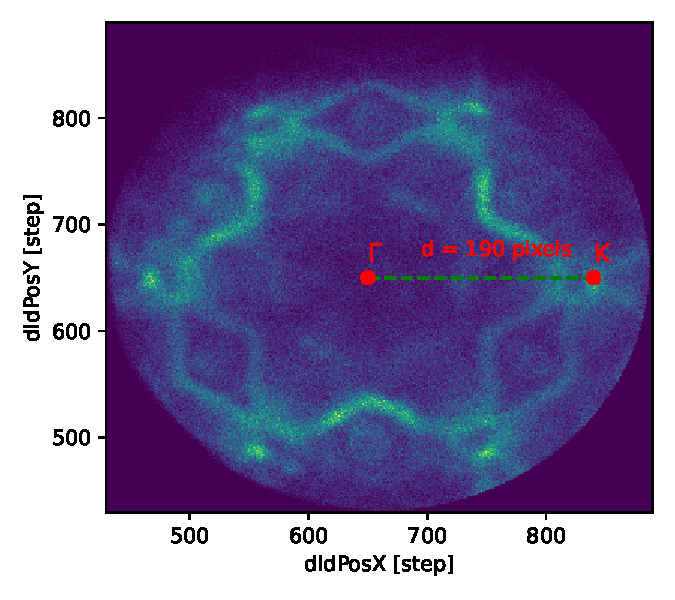
\includegraphics[width=\linewidth]{images/original_image_gamma_k.pdf}
%         \caption{Uncalibrated image with \gls{DLD} X and Y coordinates, marked with the $\Gamma$ and $K$ points, and the distance between them--$190$px.}
%         \label{fig:original-pixel-gamma-k}
%     \end{subfigure}
%     \hfill
%     % Second subfigure (Momentum-Calibrated Image)
%     \begin{subfigure}[t]{0.49\linewidth}
%         \centering
%         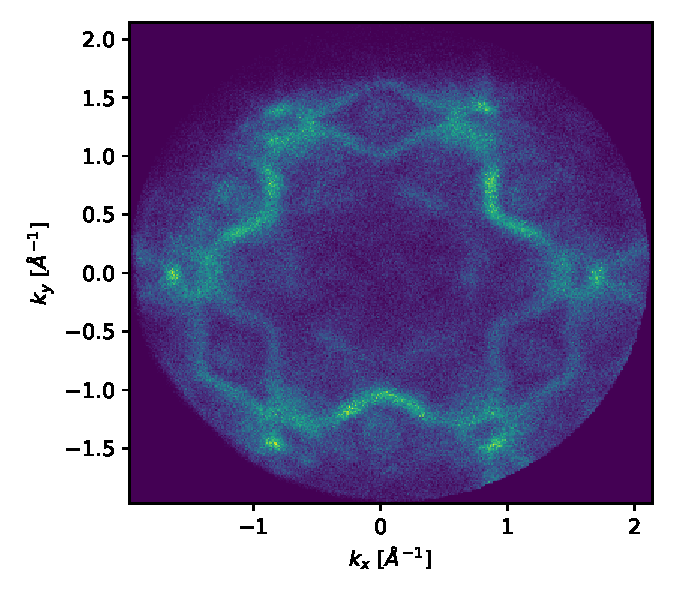
\includegraphics[width=\linewidth]{images/calibrated_momentum.pdf}
%         \caption{Calibrated momentum axes.}
%         \label{fig:calibrated-momentum}
%     \end{subfigure}
%     \caption{The detector axis and calibrated momentum axis. The left image shows the original image with the $\Gamma$ and $K$ points marked. The right image shows the calibrated momentum axes.}
% \end{figure}